\chapter{Laporan}
\section{TEORI}
\subsection{Praktek Penunjang}
Jenis-jenis variabel dan cara pemakaian variabel di kode Python
\subsubsection {Jenis-jenis variabel sebagai berikut:}
\begin{enumerate}
\item Boolean
\item Integer
\item Real
\item Karakter
\item String
\item Pointer
\item Ordinal
\end{enumerate}
\hfill \break
Cara Pemakaian variabel di kode Python
\begin{figure}[H]
		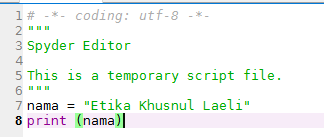
\includegraphics[width=4cm]{figures/1184065/Var1.PNG}
		\centering
		\caption{Kode perintah untuk menuliskan sebuah variabel nama}
\end{figure}
\begin{figure}[H]
		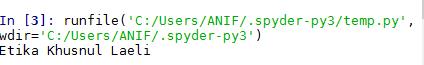
\includegraphics[width=4cm]{figures/1184065/Var2.PNG}
		\centering
		\caption{Sebuah pemberitahuan di dalam console yang meandakan bahwa kode tersebut tidak error}
\end{figure}
\begin{figure}[H]
		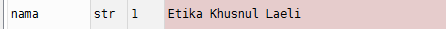
\includegraphics[width=4cm]{figures/1184065/Var3.PNG}
		\centering
		\caption{Hasil dari kode perintah yang menghasilkan variabel nama}
\end{figure}
\subsubsection{Tuliskan Kode untuk meminta input dari user dan tuliskan bagaimana output ke layar}
Berikut merupakan kode untuk meminta input dari user dan bagaimana output ke layar:
\begin{figure}[H]
		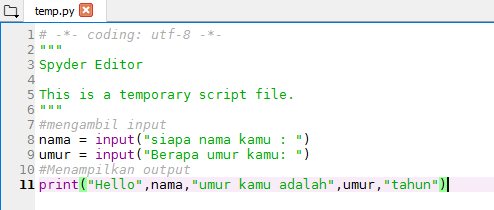
\includegraphics[width=4cm]{figures/1184065/KodeInputOutput1.PNG}
		\centering
		\caption{Kode perintah untuk meminta input dari user dan kode untuk menampilkan output ke layar}
\end{figure}
\begin{figure}[H]
		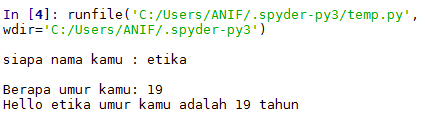
\includegraphics[width=4cm]{figures/1184065/KodeHasilInputOutput2.PNG}
		\centering
		\caption{Output dari kode perintah  }
\end{figure}
\hfill \break
\subsubsection{Tuliskan operator aritmatika, tambah, kali, kurang, bagi dan bagaimana menguubah string ke integer dan integer ke string}
\begin{figure}[H]
		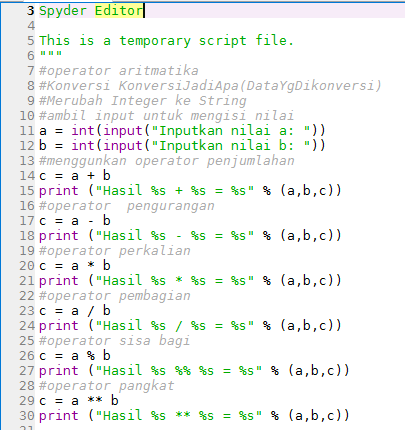
\includegraphics[width=4cm]{figures/1184065/IntKeStr.PNG}
		\centering
		\caption{Untuk menuliskan aritmatika, tambah, kali, kurang, bagi dan mengubah Integer ke string dapat menggunakan kode seperti di atas}
\end{figure}
\begin{figure}[H]
		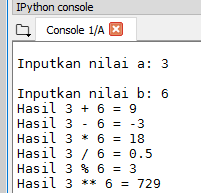
\includegraphics[width=4cm]{figures/1184065/IntKeStrHasil.PNG}
		\centering
		\caption{Hasil aritmatika dan mengubah ineger ke string}
\end{figure}
\begin{figure}[H]
		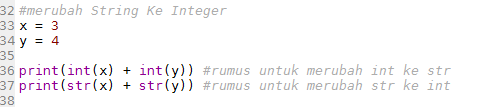
\includegraphics[width=4cm]{figures/1184065/StrKeIntNew.PNG}
		\centering
		\caption{Koding untuk mengubah string ke integer}
\end{figure}
\begin{figure}[H]
		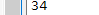
\includegraphics[width=4cm]{figures/1184065/StrkeIntHasil.PNG}
		\centering
		\caption{Hasil nya yaitu karena string di tambah integer tidak bisa di eksekusi, sehingga bisa diakali dengan kode seperti diatas. Yang nanti outputnya antara string satu dan string dua itu disatukan buka di tambah.}
\end{figure}
\subsubsection{Tuliskan dan jelaskan untuk sintak perulangan jenis-jenisnya, contoh kode dan cara pakainya di python }
\begin{enumerate}
\item Perulangan For
\hfill \break
Perulangan for sering disebut sebagai counted loop atau perulangan yang terhitung. Untuk perulangan for biasanya digunakan untuk mengulangi kode yang sudah diketahui berapa banyak perulangannya.
\begin{figure}[H]
		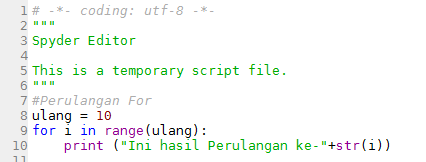
\includegraphics[width=4cm]{figures/1184065/PerFor.PNG}
		\centering
		\caption{untuk koding perulangan  For bisa menggunakan kode seperti diatas}
\end{figure}
\begin{figure}[H]
		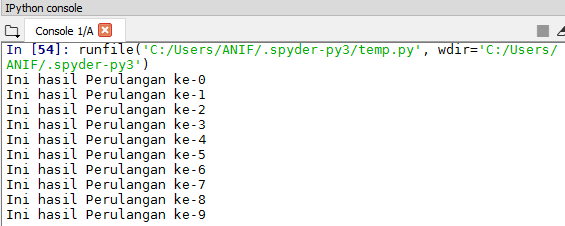
\includegraphics[width=4cm]{figures/1184065/PerForHasil.PNG}
		\centering
		\caption{Hasil For akan berhenti pada urutan ke-9 karena perulangan telah di setting seperti kode ditas}
\end{figure}
\item Perulangan While
\hfill \break
Sedangkan perulangan While sering sering disebut sebagai uncounted loop atau perulangan yang tidak terhitung. Sementara while untuk perulangannya mempunyai syarat dan tidak tentu berapa banyak perulangannya
\begin{figure}[H]
		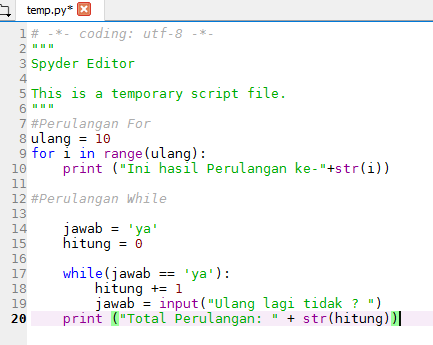
\includegraphics[width=4cm]{figures/1184065/PerWhile.PNG}
		\centering
		\caption{Untuk koding while kita dapat lihat seperti gambar diatas}
\end{figure}
\begin{figure}[H]
		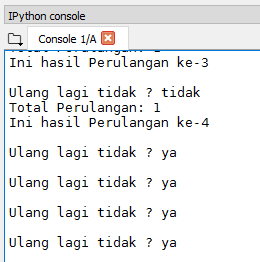
\includegraphics[width=4cm]{figures/1184065/PerWhileHasil.PNG}
		\centering
		\caption{untuk hasil while akan berhenti ketika kita menjawab tidak}
\end{figure}
\subsubsection{Tuliskan dan jelasknan cara pakai sintak untuk memilih kondisi dan bagaimana contoh sintak kondisi di dalam kondisi}
\begin{enumerate}
\item Penggunaan if
\hfill \break
Kondisi if digunakan untuk mengekseskusi kode jika kondisinya itu bernilai benar atau true.
\begin{figure}[H]
		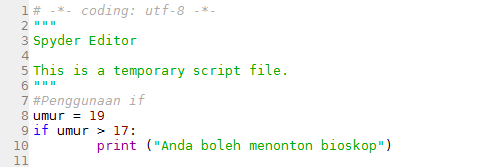
\includegraphics[width=4cm]{figures/1184065/IF.PNG}
		\centering
		\caption{Koding untuk kondisi IF}
\end{figure}
\begin{figure}[H]
		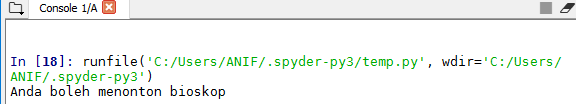
\includegraphics[width=4cm]{figures/1184065/IF_Hasil.PNG}
		\centering
		\caption{Hasil untuk kondisi IF akan dieksekusi jika bernilai true. seperti gambar ditas}
\end{figure}
\end{enumerate}
\item Penggunaan if else
\hfill \break
Kondisi if else yaitu dimana kondisi jika pernyataan true maka kode dalam if akan dieksekusi, tapi jika kondisi berniai false maka kode akan di eksekusi di else.
\begin{figure}[H]
		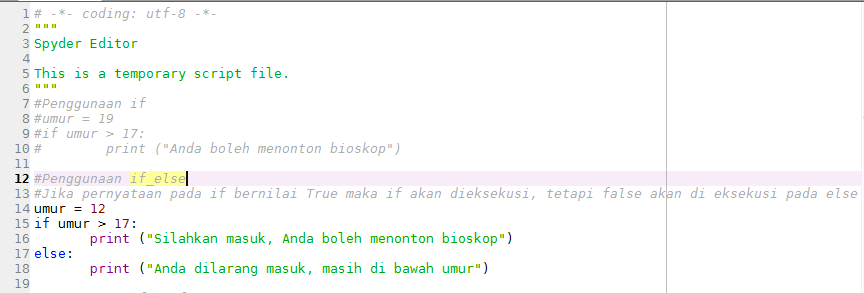
\includegraphics[width=4cm]{figures/1184065/IF_ELSE.PNG}
		\centering
		\caption{Koding untuk kondisi if else}
\end{figure}
\begin{figure}[H]
		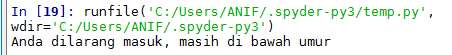
\includegraphics[width=4cm]{figures/1184065/IF_ELSE_Hasil.PNG}
		\centering
		\caption{Hasil koding dari kondisi if else yaitu jika kondisi bernilai true akan dieksekusi dan jika kondisi bernilai false akan tetap di eksekusi pada else}
\end{figure}
\item Penggunaan if elif else
\hfill \break
Untuk kondisi if elif else atau yang sering disebut kondisi didalam kondisi yang mana tidak hanya satu kondisi yang nilainya true bisa juga terdpat dua kondisi atau lebih yang bernilai true
\begin{figure}[H]
		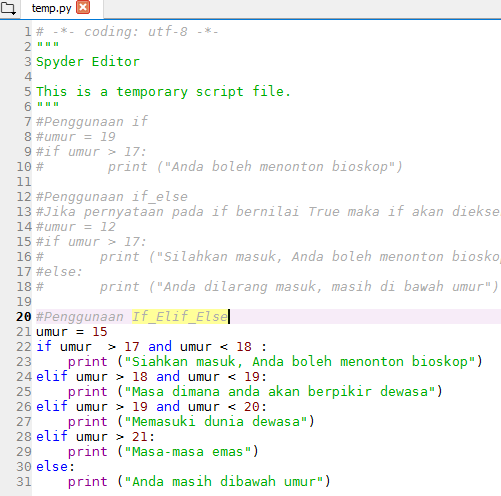
\includegraphics[width=4cm]{figures/1184065/IF_ELIF_ELSE.PNG}
		\centering
		\caption{Kode untuk if elif else}
\end{figure}
\begin{figure}[H]
		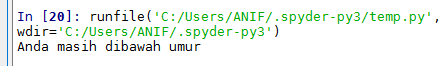
\includegraphics[width=4cm]{figures/1184065/IF_ELIF_ELSE_HASIL.PNG}
		\centering
		\caption{untuk outputan dari koding if elif else karena untuk masuk ke dalam sebuah bisokop harus berumur leih dari 17 tahun maka kodisi  yang di outputkan adalah else}
\end{figure}
\hfill \break
\end{enumerate}
\subsubsection{Tuliskan jenis error apa saja yang sering ditemui di python dalam mngerjakan syntak di atas dan bagaimana cara mengatasinya}
\begin{figure}[H]
		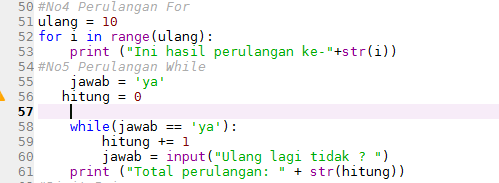
\includegraphics[width=4cm]{figures/1184065/SintakError.PNG}
		\centering
		\caption{Koding pada sintak yang salah}
\end{figure}
\begin{figure}[H]
		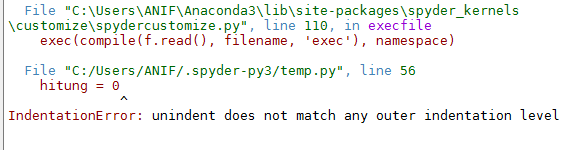
\includegraphics[width=4cm]{figures/1184065/SintakPemberitahuanError.PNG}
		\centering
		\caption{Jika sitak salah akan diberikan sebuah Pemberitahuan Error}
\end{figure}
\begin{figure}[H]
		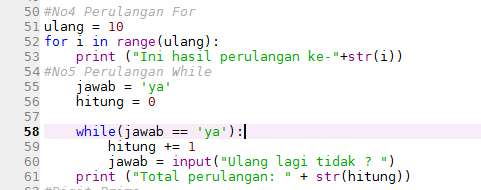
\includegraphics[width=4cm]{figures/1184065/SintakErrorMenangani.PNG}
		\centering
		\caption{Nah untuk menangani Error kiat bisa baca dari pemberitahuan yaitu karena untuk sintak hitung kurang maju ke depan}
\end{figure}
\begin{figure}[H]
		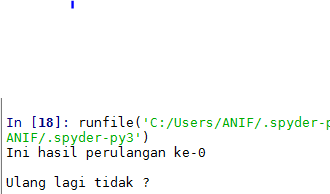
\includegraphics[width=4cm]{figures/1184065/SintakHasilMenanganiError.PNG}
		\centering
		\caption{Setelah tahu errornya maka sintak tersebut akan bisa dieksekusi kembali}
\end{figure}
\subsubsection{Tuliskan dan Jelaskan cara memakai Try Except}
Try Except merupakan salah satu bentuk penanganan error di bahasa pemrograman python
\begin{enumerate}
\item Menangani error pembagian nol
\hfill \break
Kode yang membagi suatu angka dengan sebuah nol maka program akan error. Sehingga kita kurung dengan try..except, kemudian keluarkan error nya yang tertangkap error oleh except.
\item Menangani error pembacaan file
\hfill \break
di dalam kode ini kita akan mencoba untuk  menangkap dua error yang dikurung oleh try except.
\item Mengenal Finally
\hfill \break
Finally merupakan kode yang menangani apabila terjadi suatu error ataupun kode yang harus dieksekusi.
\item Mengenal Raise
\hfill \break
Raise juga digunakan untuk membantu menangani error. Raise biasanya digunakan dengan if else atau pemeriksaan lainnya.
\end{enumerate}
\section{KETRAMPILAN PEMROGAMAN}
\lstinputlisting[language=Python]{src/NPM1.py}
\lstinputlisting[language=Python]{src/NPM2.py}
\lstinputlisting[language=Python]{src/NPM3.py}
\lstinputlisting[language=Python]{src/NPM4.py}
\lstinputlisting[language=Python]{src/NPM5.py}
\lstinputlisting[language=Python]{src/NPM6.py}
\lstinputlisting[language=Python]{src/NPM7.py}
\lstinputlisting[language=Python]{src/NPM8.py}
\lstinputlisting[language=Python]{src/NPM9.py}
\lstinputlisting[language=Python]{src/NPM10.py}
\lstinputlisting[language=Python]{src/NPM11.py}
\hfill\break
\section{Ketrampilan Penanganan Error}
\lstinputlisting[language=Python]{src/2err.py}
\subsection{Penanganan Error}
\subsubsection{Penanganan Error yang didapat dari mengerjakan praktek dan jelaskan cara penanganannya}
\begin{enumerate}
\item Untuk error yang di dapat tadi salah bahasa yang digunakan dalam bahasa pemrograman, yang harusnya bahasa inggris malah menggunakan bahasa indonesia. Tapi sudah di atasi kembali menjadi sintak yang benar dan bisa di eksekusi.
\item Penulisan scrip yang tidak teratur menyebabkan program tidak bisa di eksekusi, menanganinya dengan cara script di teliti ulang
\item Salah memasukan inputan gambar, diatasi dengan cara memasukan gambar yang benar.
\end{enumerate}
\subsubsection{Membuat file 2er.py dan mengisinya dengan script pengisian variabel sebagai string dan pengisian variabel sebagai integer. Kemudian jumlahkan antara variabel integerdan string dan tngkap jenis errornya, gunakan try except untuk menunjukan error tersebut dengan bahasa indonesia}
\lstinputlisting[language=Python]{src/2err.py}
\begin{figure}[H]
		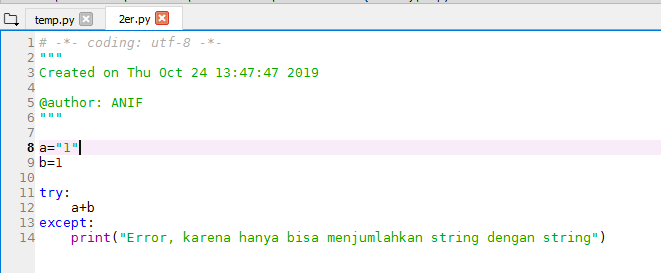
\includegraphics[width=4cm]{figures/1184065/2er.PNG}
		\centering
		\caption{Kodingan Variabel sebagai string dan variabel sebagai integer }
		\begin{figure}[H]
		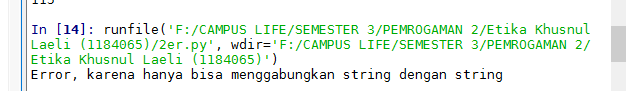
\includegraphics[width=4cm]{figures/1184065/2erError.PNG}
		\centering
		\caption{Error}
\end{figure}
\end{figure}
